
\chapter{Anforderungsanalyse}
\label{chapter_Anforderungsanalyse}
Das Ziel dieser Arbeit ist es, eine Steuereinheit für einen Teststand zu entwickeln, der die Messung der Degradation von optoelektronischen Sendern ermöglicht. In diesem Kapitel wird zunächst das Szenario aus dem sich die Notwendigkeit des Systems ergibt näher beschrieben. Dann erfolgt eine Analyse der beteiligten Akteure und im Anschluss werden die Anforderungen definiert.

\section{Szenario}
Ein Unternehmen stellt verschiedene optoelektronische Sensoren her. Zur Sicherstellung der Zuverlässigkeit der verwendeten \acp{LED} sollen diese mittels eines automatisierten Teststandes bezüglich ihres Degradationsverhaltens qualifiziert werden.


\begin{figure}[H]
\begin{center}
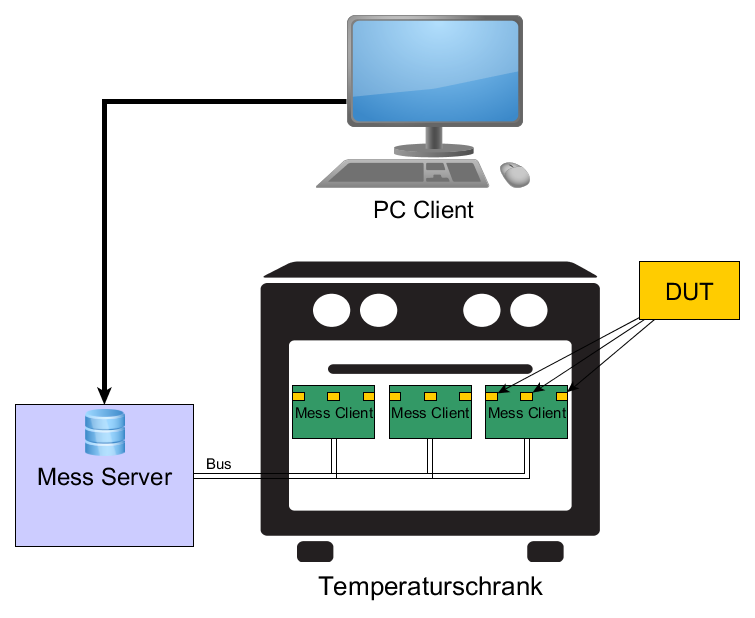
\includegraphics[width=0.6\textwidth]{img/general/Szenario.png}
\caption{Szenario}
\label{figure_Szenario}
\end{center}
\end{figure}

Der Teststand hat den in Abbildung \ref{figure_Szenario} zu sehenden Aufbau.
In einem Temperaturschrank befinden sich mehrere Mess-Clients. An diesen Mess-Clients sind jeweils 64 \acp{DUT} fest angeschlossen, bei denen das Degradationsverhalten aufgezeichnet werden soll.
Die Mess-Clients sind über einen Bus mit einem außerhalb des Temperaturschrankes befindlichen Mess-Server verbunden, welcher zyklisch Messdaten von den Mess-Clients abruft und alle anfallenden Daten in einer Datenbank speichert.\\
Von einem PC-Client kann auf den Mess-Server zugegriffen  werden, um die Messdaten zu beziehen und grafisch auszuwerten.\\

\section{Analyse}

Die Akteure des Systems sind der Mess-Server, Mess-Client und PC-Client. Im Zuge dieser Arbeit soll der Mess-Server realisiert werden. Wobei die Interaktionsfähigkeit mit den anderen Akteuren sichergestellt werden muss.


\subsection{Mess-Server}
\label{section_Mess-Server}

\begin{figure}[H]
\begin{center}
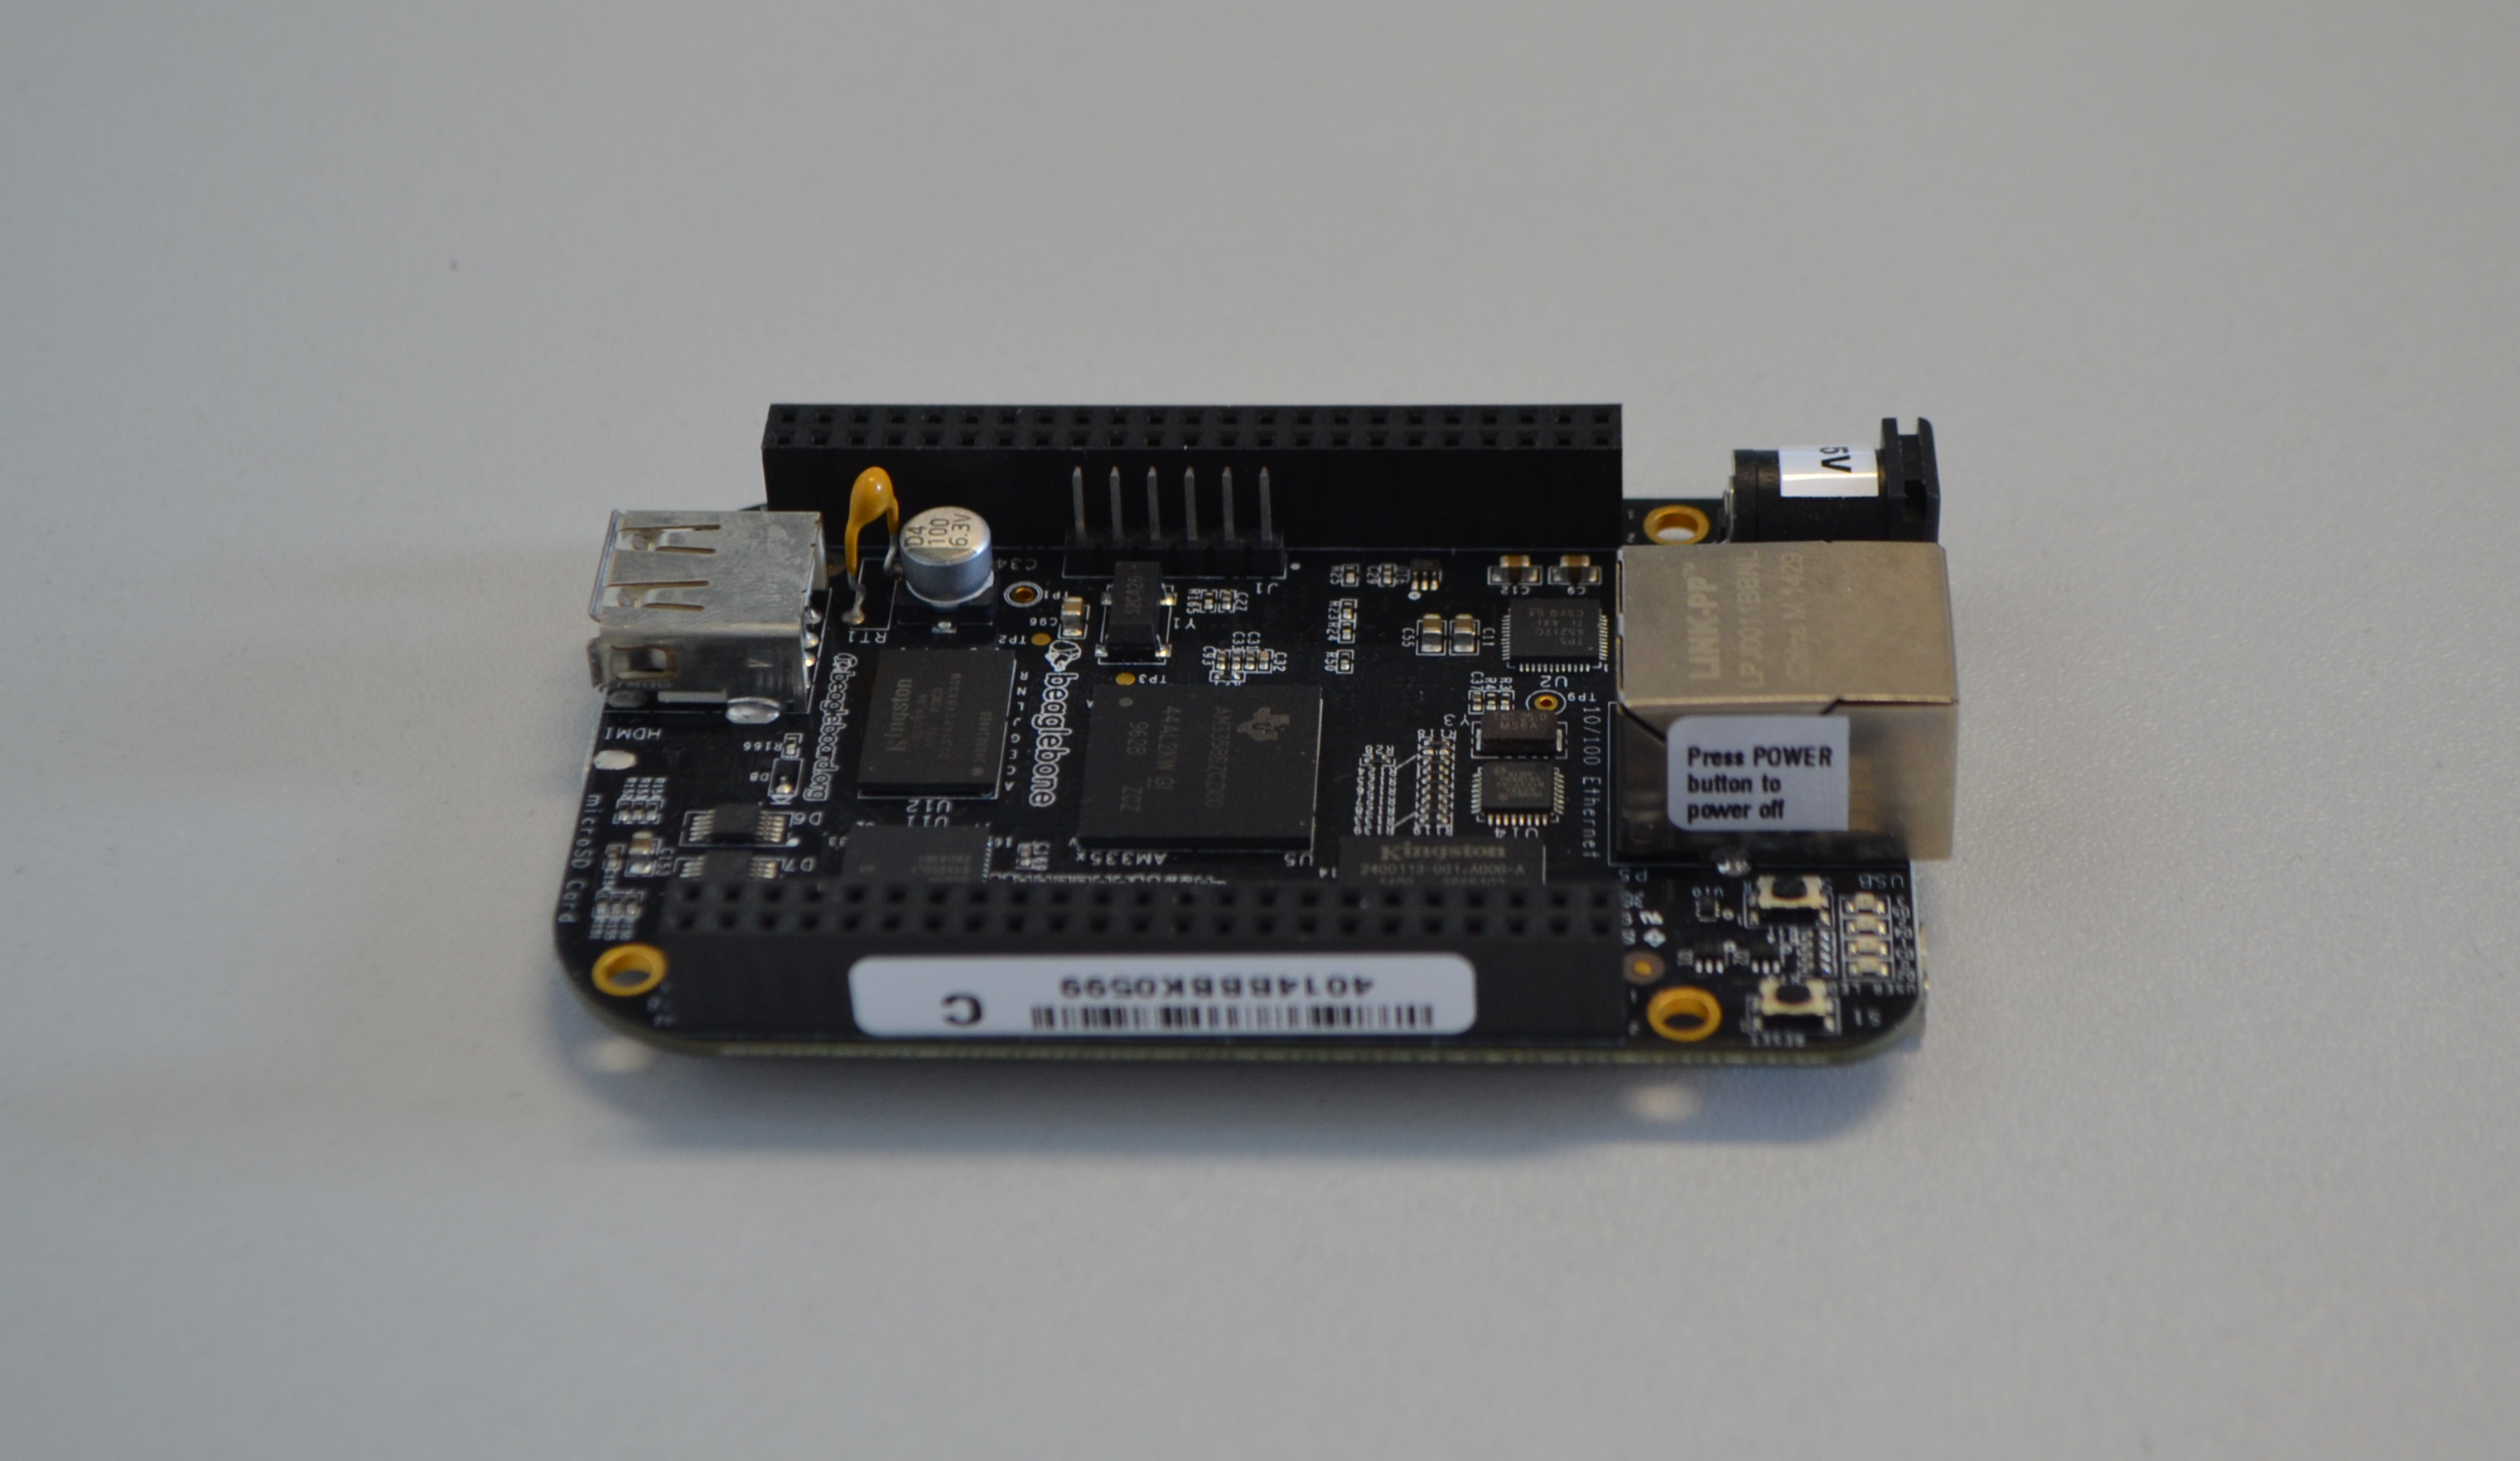
\includegraphics[width=0.6\textwidth]{img/general/BeagleBoneBlack.png}
\caption{BeagleBone Black}
\label{figure_Beagleboneblack}
\end{center}
\end{figure}


Als Mess-Server wird ein BeagleBone Black von Texas Instruments eingesetzt (siehe Abbildung \ref{figure_Beagleboneblack}). Dabei handelt es sich um einen kostengünstigen Einplatinencomputer mit offener Hardware. Dadurch ist es möglich, das BeagleBone Black auf individuelle Anforderungen anzupassen und selbst herzustellen. Auch gibt es eine große Community, die ständig die Entwicklung vorantreibt.
Die aktuelle Revision C arbeitet mit einem AM335x 1GHz ARM® Cortex-A8 Prozessor, verfügt über 512MB DDR3 RAM und 4GB 8-bit eMMC internen Flash Speicher. Als Spannungsversorgung dient ein 5V 2A Netzteil. Trotz der Kompaktheit des BeagleBone Black, bietet er ein ausreichendes Maß an Performance.\\
Auf ihm kommt ein eingebettetes Debian-GNU/Linux Betriebssystem (siehe Abschnitt \ref{section_EmbeddedLinux}) zum Einsatz. Wie auch J. Schröder et al. (vgl. \cite{schroeder2009embedded}) sagt, ist es dadurch möglich die umfangreichen Linux-Funktionen wie die Paketverwaltung zu nutzen. Es bietet auch den Vorteil, dass eine große Ähnlichkeit zu PC-Distributionen wie Ubuntu besteht und somit die Linux Mechanismen einfach nutzbar sind. So kann das RS232 Interface beispielsweise wie eine normale Datei beschrieben und gelesen werden (siehe Abschnitt \ref{section_EmbeddedLinux}).

Für die Kommunikation mit den anderen Akteuren im System muss ein RS232 Bussystem und eine Ethernet Schnittstelle realisiert werden. Des Weiteren soll ein MySQL Datenbankserver auf dem Mess-Server die effiziente Verwaltung von Daten übernehmen. Zusätzlich soll eine Statusanzeige zur Überwachung des Mess-Servers entwickelt werden.


\subsection{Mess-Client}
\label{section_Mess-Client}
 
 \begin{figure}[H]
\minipage{0.43\textwidth}
  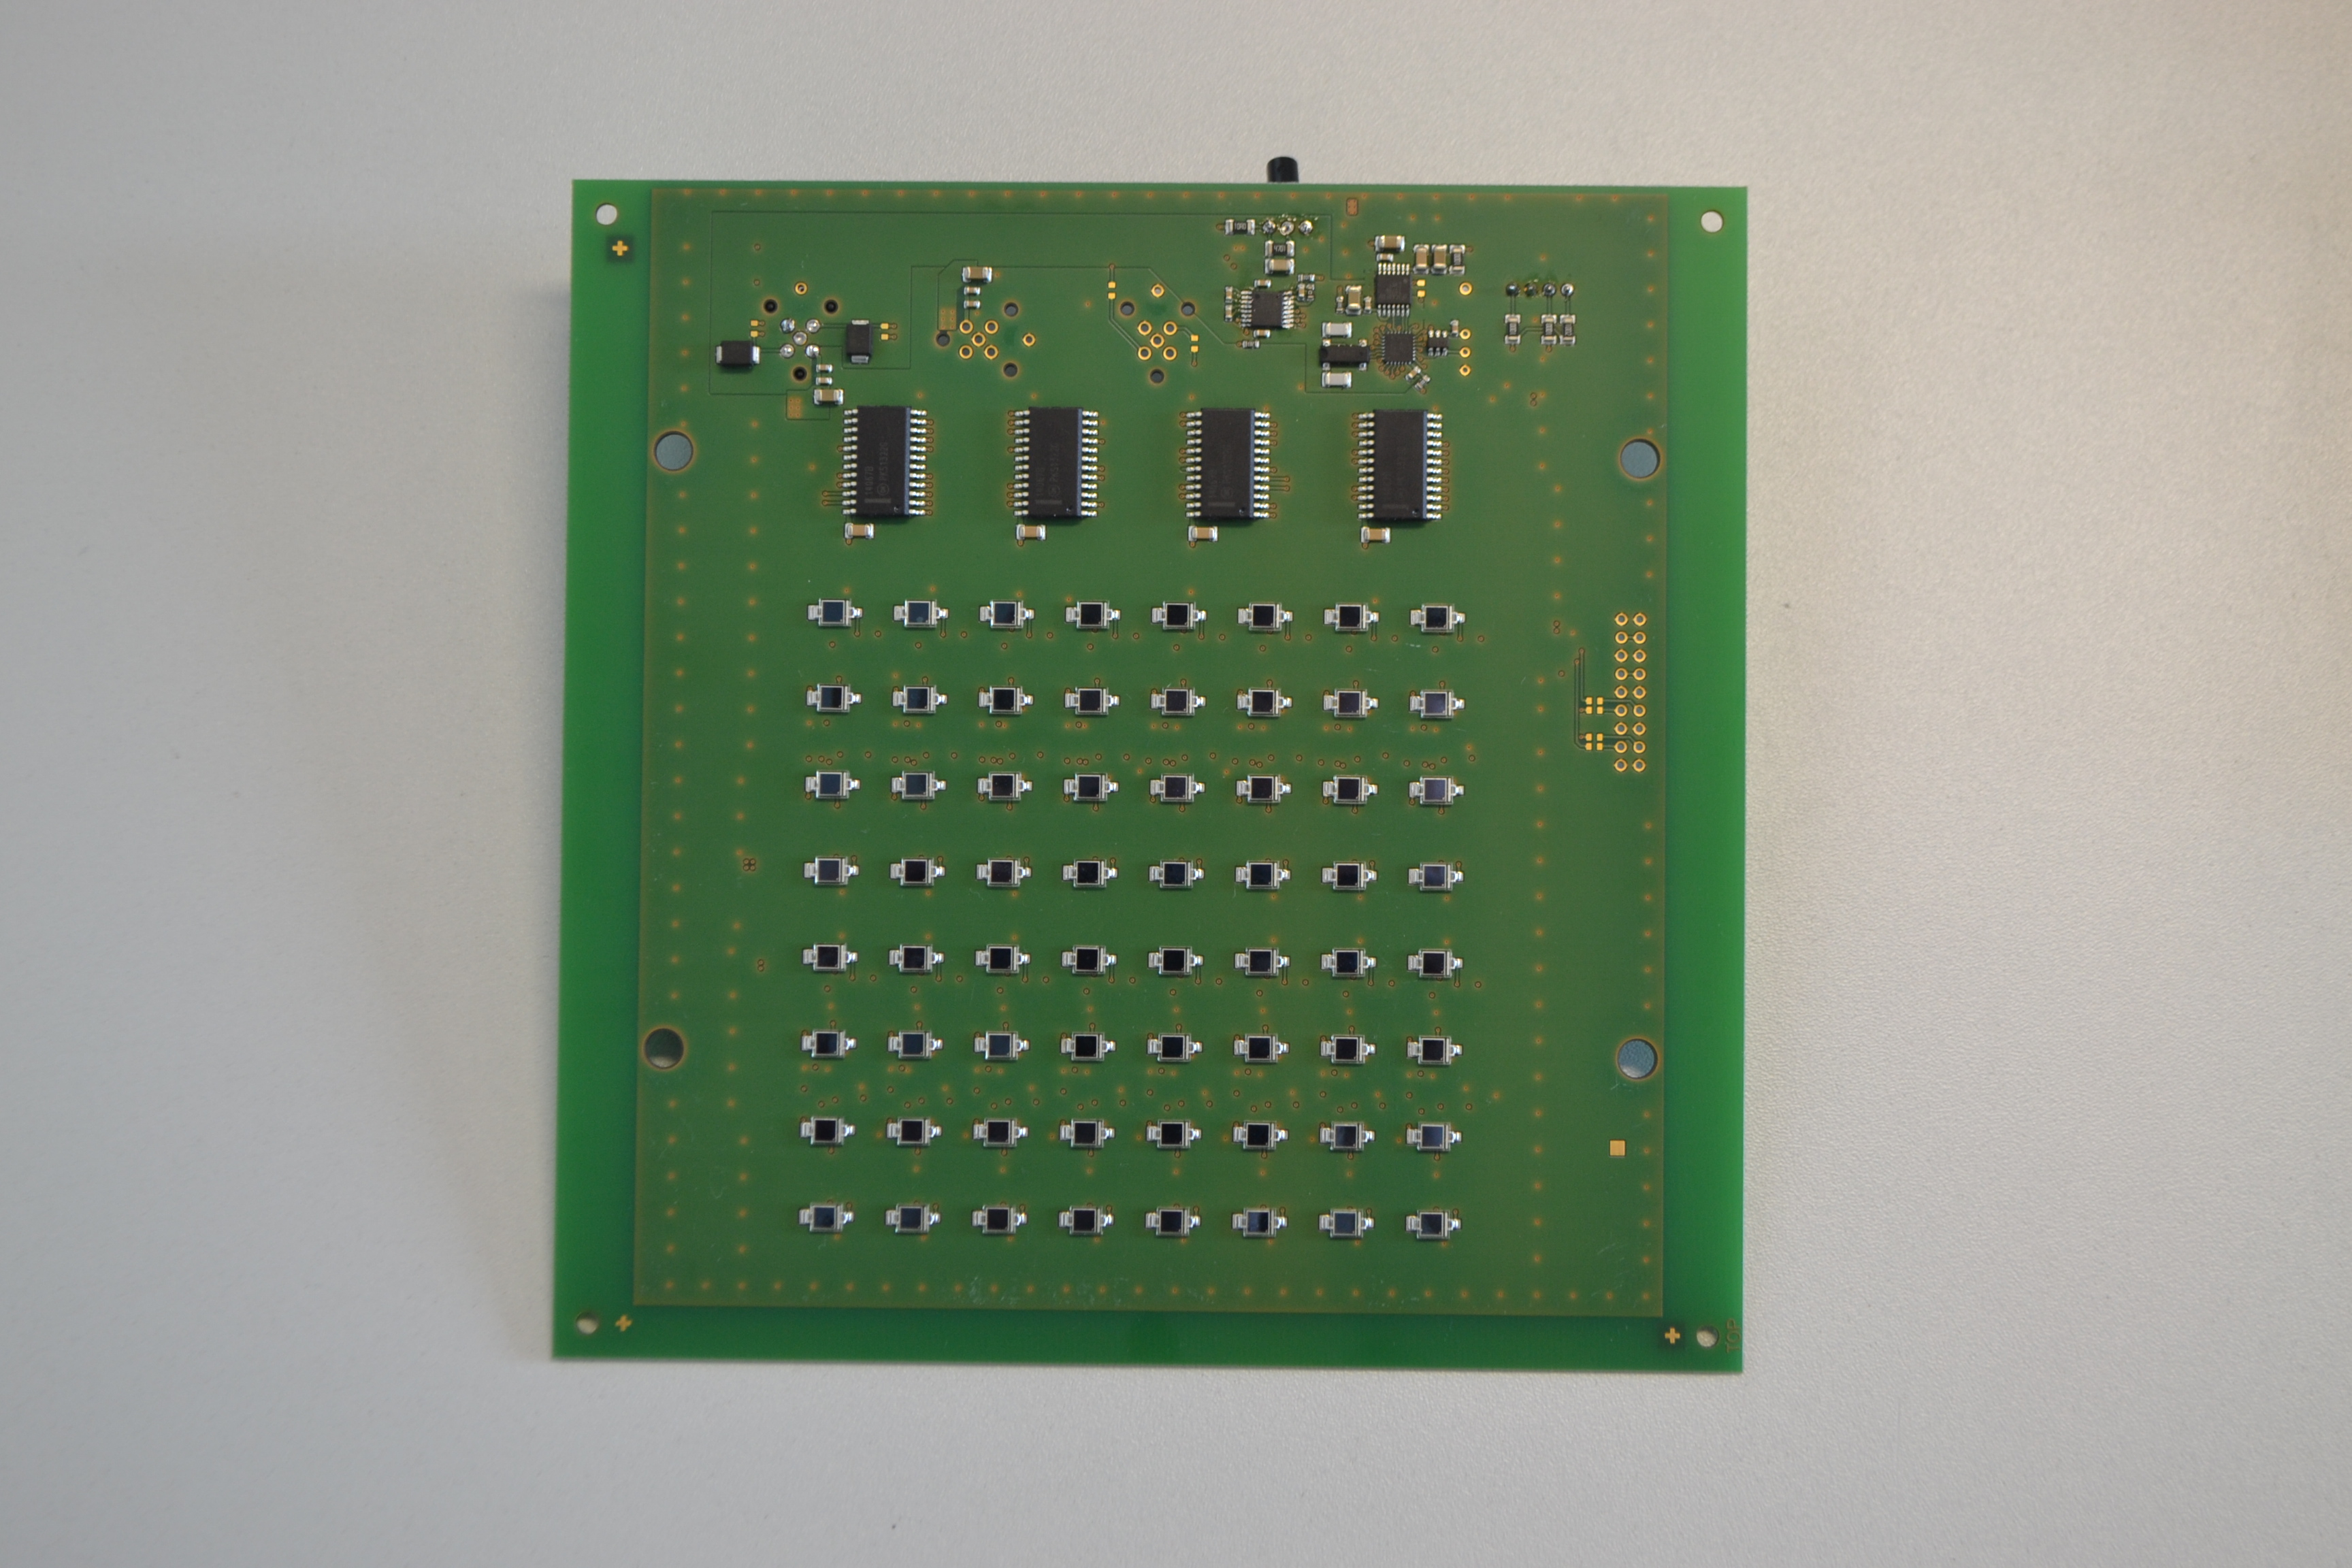
\includegraphics[width=\linewidth]{img/general/DegraBoardTop.jpg}
  \caption{Mess-Client Oberseite}\label{figure_DegraBoardTop}
\endminipage\hfill
\minipage{0.43\textwidth}%
  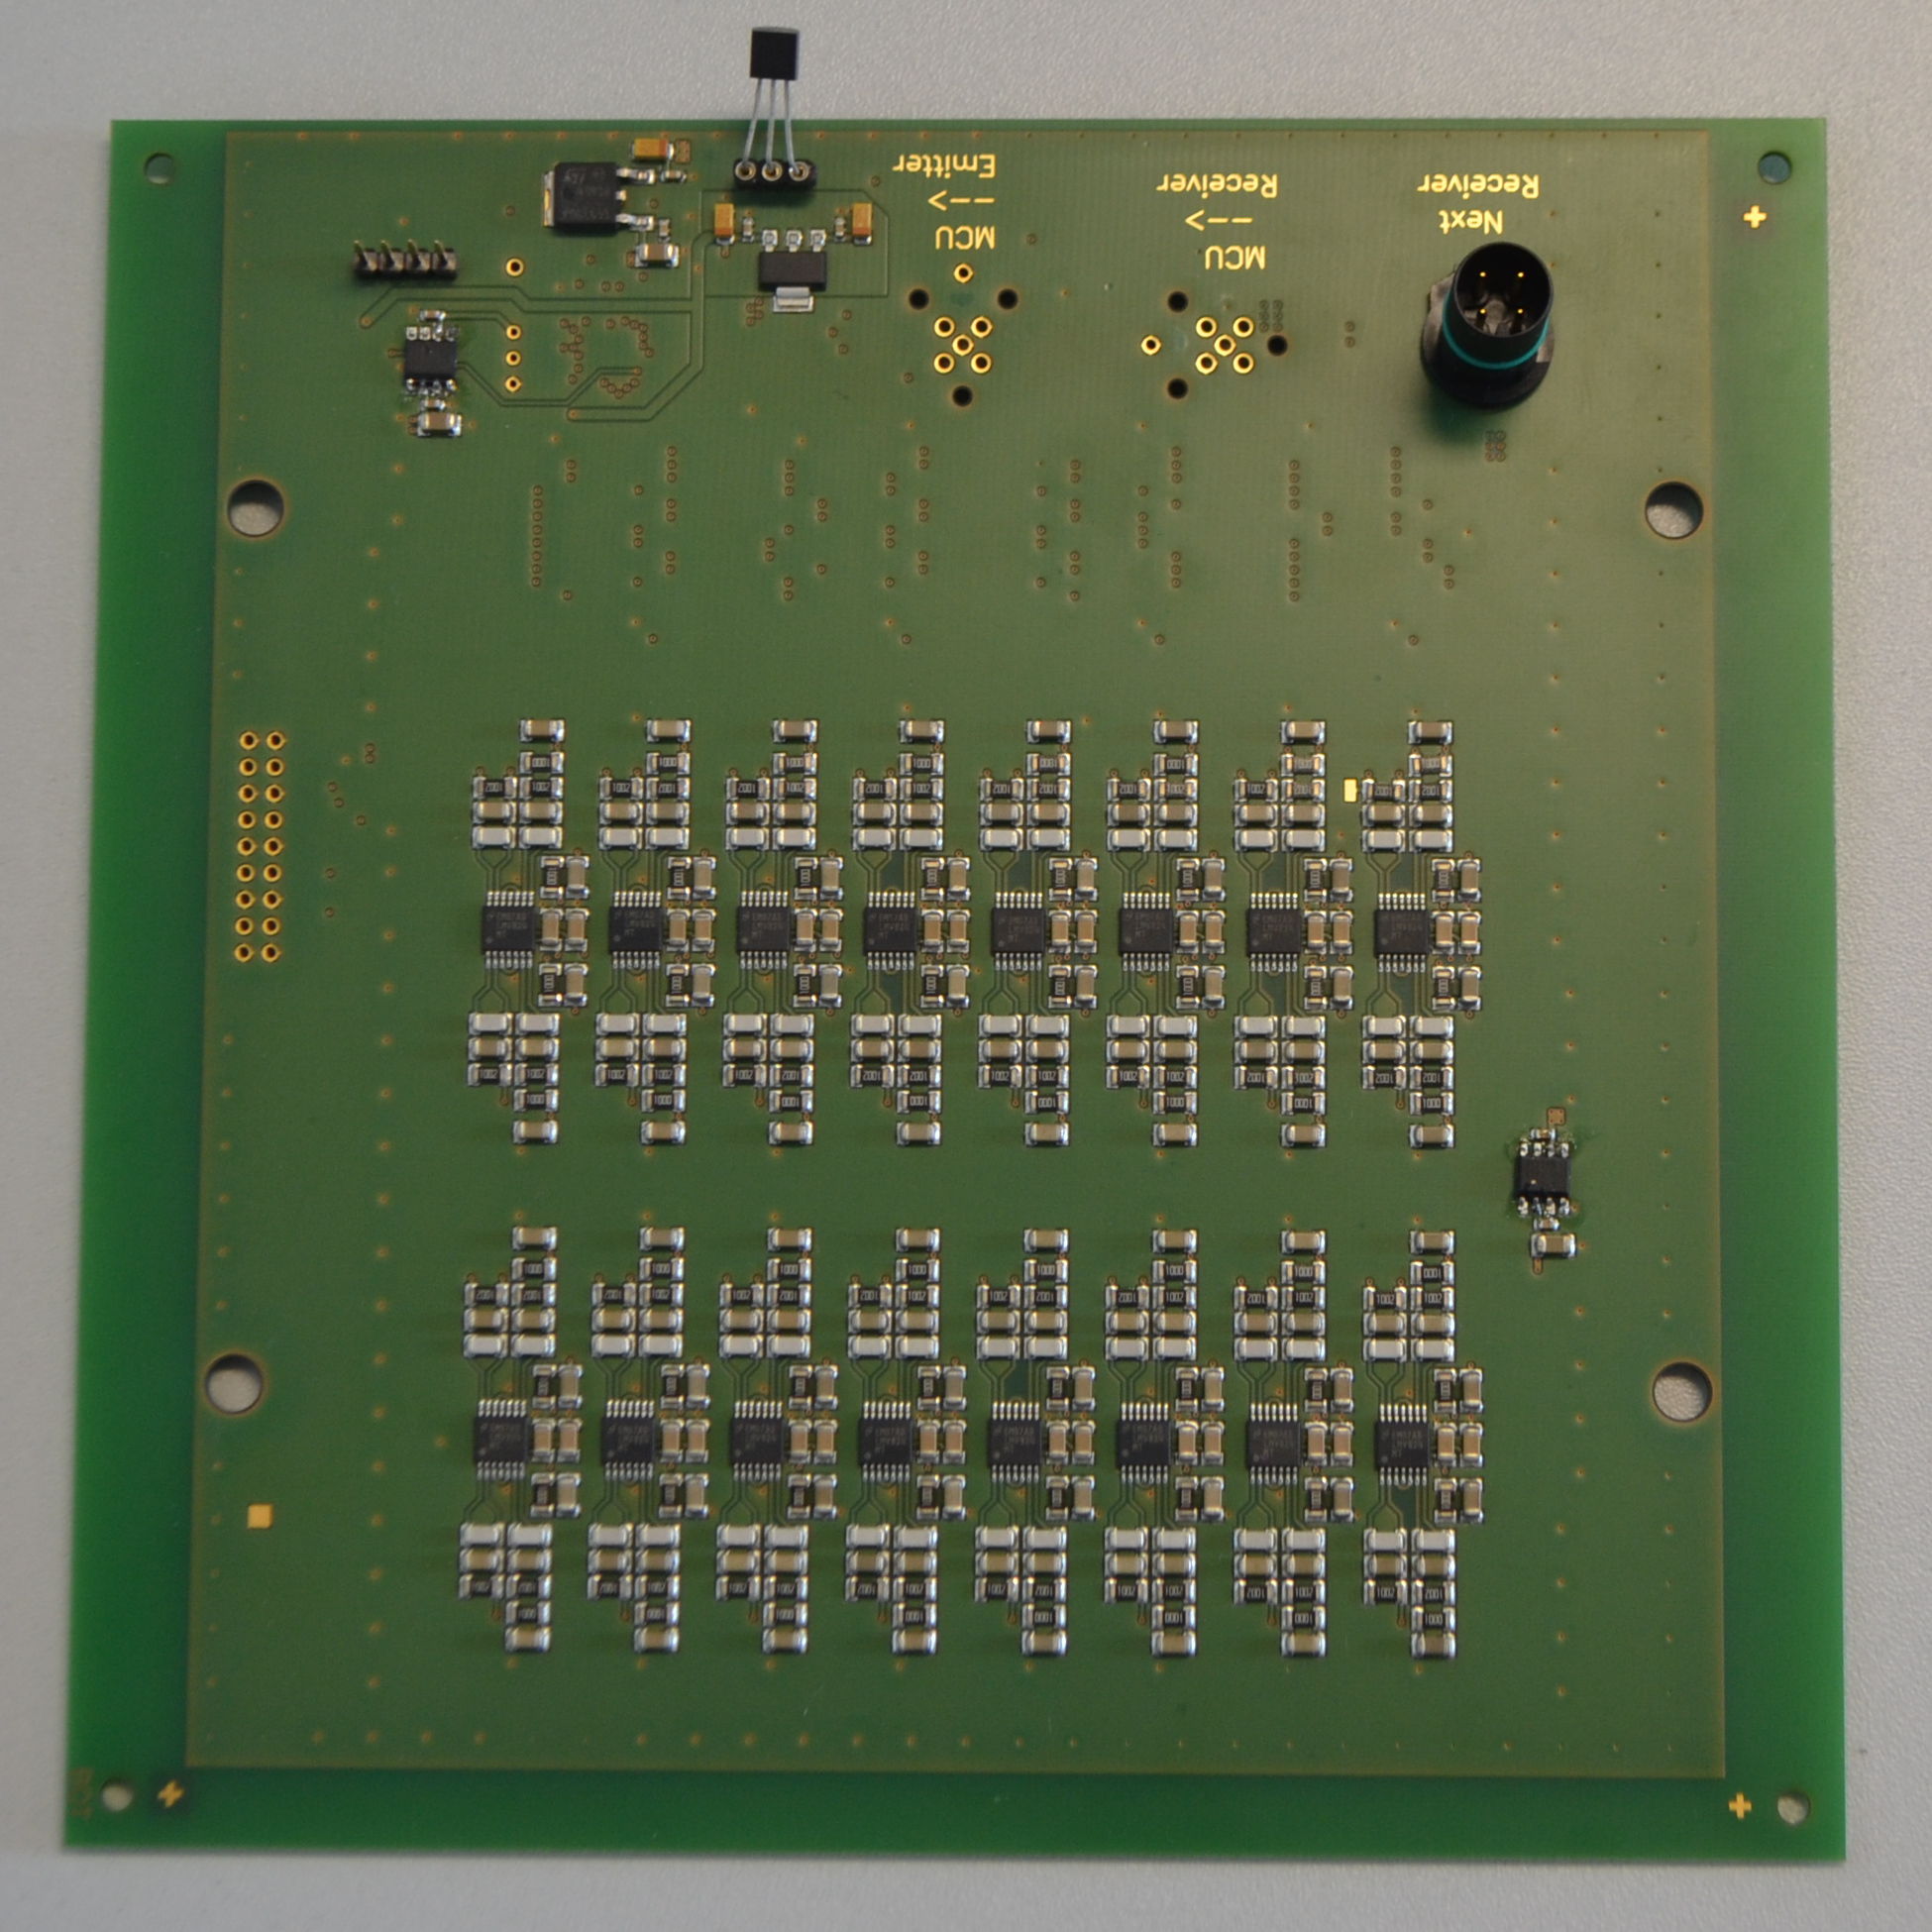
\includegraphics[width=\linewidth]{img/general/DegraBoardBottom.jpg}
  \caption{Mess-Client Unterseite}\label{figure_DegraBoardBottom}
\endminipage
\end{figure}

Ein Mess-Client (auch: Degradations Board) ist eine Leiterplatte auf der sich 64 optische Empfängern zur Messung von optischen Signalen befinden (siehe Abbildung \ref{figure_DegraBoardBottom} und \ref{figure_DegraBoardTop}). Auf jedem Mess-Client können somit bis zu 64 Prüfobjekte befestigt werden. In zyklischen Abständen werden mittels eines Mikrocontrollers die Messdaten der Prüfobjekte aufgenommen und über eine RS232-Schnittstelle zur Verfügung gestellt.\ 

Für die Konfiguration speichert der Mess-Client die Parameter in einem persistenten Speicher. Folgende Parameter stehen dabei zur Verfügung:

\textbf{Name}\\
Für die Identifikation hat jeder Mess-Client einen Namen der aus maximal 30 Zeichen bestehen kann. Er dient vor allem für die Identifizierung der verschiedenen Mess-Clients.\ 

\textbf{RS232 Adresse}\\
Um über die RS232 Schnittstelle ansprechbar zu sein, verfügt jeder Mess-Client über eine Adresse. Lediglich wenn eine Nachricht diese Adresse beinhaltet, reagiert der Mess-Client. Die Adresse ist mit 7 Bit aufgelöst und bildet einen Adressraum von 128 Adressen.\ 

\textbf{Messintervalle}\\
Zur Steuerung der Intervalle, in denen Messwerte vom Mess-Server aufgezeichnet werden sollen, speichert der Mess-Client diese Informationen. Es ist möglich, Messintervalle für drei Zeiträume zu definieren.



\begin{figure}[H]
\begin{center}
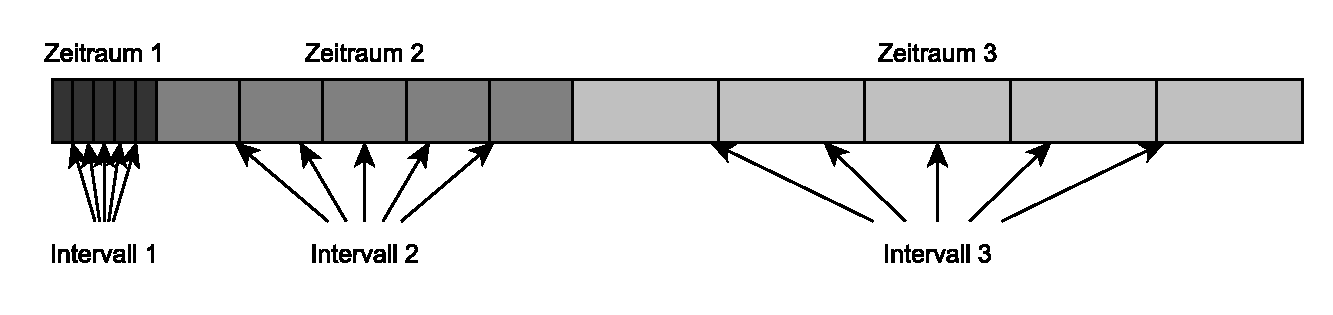
\includegraphics[width=0.8\textwidth]{img/general/Messintervalle.pdf}
\caption{Messintervalle}
\label{figure_Messintervalle}
\end{center}
\end{figure}

In Abbildung \ref{figure_Messintervalle} ist ist die Unterteilung der Zeiträume und Messintervalle zu sehen. Jeder definierte Zeitraum hat seine eigenes Messintervall, welches den Abstand zwischen den Messdatenabfragen bestimmt.\ 

\textbf{Pulsmuster}\\
Der Mess-Client steuert die Prüfobjekte mit einem Pulsmuster (englisch: pulse pattern) an. Dieses Muster ist konfigurierbar und wird an die unterschiedlichen Prüfobjekte angepasst. Ein Pulsmuster besteht aus bis zu 20 verschiedenen Pulsen, die periodisch wiederholt werden. Ein Puls besteht dabei aus einer Pulsperiode und einer Pulsbreite. In Abbildung \ref{figure_Pulsepattern} ist ein Pulsperiode/Pulsbreiten-Paar zu sehen.\\



\begin{figure}[H]
\begin{center}
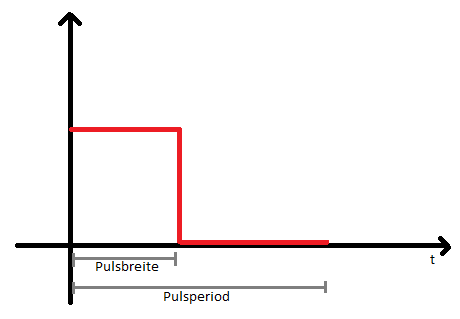
\includegraphics[width=0.5\textwidth]{img/general/PulseMuster.png}
\caption{Pulsperioden/Pulsbreiten-Paar}
\label{figure_Pulsepattern}
\end{center}
\end{figure}


\subsection{PC-Client}
\label{section_PC-Client}
Der PC-Client stellt eine Qt Desktop-Anwendung mit einer Benutzeroberfläche zur Auswertung der Messdaten dar, die nicht im Rahmen dieser Bachelorarbeit entwickelt wird. Über die Ethernet Schnittstelle ruft er die Messdaten von dem Mess-Server ab und bereitet sie zur genaueren Auswertung grafisch auf.\\
Außerdem werden über die Desktop-Anwendung die Mess-Clients parametriert. Dafür wird ein Mess-Client lokal über die RS232 Schnittstelle an den PC-Client angeschlossen. Dies ist notwendig, da einige Parameter in Abhängigkeit von den Prüfobjekten eingestellt werden müssen.\\
Im laufenden Betrieb können die Mess-Clients von einem PC-Client aus per Fernzugriff verwaltet werden. Dies beinhaltet die Änderung der Parametrierung und das Auslesen der Messdaten. Dafür werden auf dem Mess-Client persistent Parameter gespeichert, welche über die RS232 Schnittstelle geschrieben und ausgelesen werden können.



\section{Anforderungen}
Folgende Hauptanforderungen werden an das System gestellt:
\begin{itemize}
\item Individuelle Parametrierung der Prüfobjekte
\item Automatische Erfassung der Messdaten
\item Fernzugriff auf den Mess-Server zum Abrufen der Messdaten
\end{itemize}
\ 

\textbf{Individuelle Parametrierung der Prüfobjekte}\\
Immer 64 Prüfobjekte befinden sich auf einem Mess-Client. Dabei sollen verschiedene Parameter für die Prüfobjekte berücksichtigt werden. 
Zum Einen sollen die Intervalle in denen Messwerte aufgenommen werden konfigurierbar sein. Dies soll in mindestens 3 verschiedenen Intervallen möglich sein. In Tabelle \ref{table_Intervalle} ist ein Beispiel für die Messintervalle zu sehen. 

 
\begin{table}[H]
\begin{center}
\begin{tabular}{|l|l|}\hline
Zeitraum & Zeit zwischen Messungen \\ \hline
1. Woche & 12 Stunden\\ 
2. bis 4. Woche & 2 Tage\\ 
ab 5. Woche & 7 Tage\\ \hline
\end{tabular}
\caption{Beispiel: Intervalle}
\label{table_Intervalle}
\end{center}
\end{table}



Zum Anderen soll für jeden Mess-Client ein Pulsepattern definierbar sein. Dieses Pulsepattern wird dann als Ansteuerungssignal für die \acp{DUT} verwendet.

\textbf{Automatische Erfassung der Messdaten}\\
Die Messdaten der \acp{DUT} sollen zyklisch erfasst werden. Es soll die derzeitige Temperatur im Ofen, der gemessene Wert des Sensors und ein Zeitstempel gespeichert werden. Dabei sollen, wie bereits erwähnt, die Intervalle zwischen den Messungen konfigurierbar sein.\\
Für den einfachen und effizienten Zugriff auf die Daten sollen sie in einer \ac{SQL} Datenbank abgelegt werden. Dafür ist eine Kommunikationsschnittstelle zwischen der Datenbank und den Mess-Clients erforderlich, welche über den Mess-Server realisiert wird.

\textbf{Fernzugriff auf den Mess-Server}\\
Zur Auswertung der Messdaten soll es möglich sein, von einem PC-Arbeitsplatz aus eine Verbindung zu dem Mess-Server aufzubauen. Die Messdaten sollen grafisch auf dem PC-Client zur Auswertung aufbereitet werden.
Auch soll ein Tunnelmodus direkten Zugriff von einem PC-Client auf einem Mess-Client ermöglichen. Dabei sollen die Parameter des Mess-Clients verändert werden können.

Diese Basis-Anforderungen und einige zusätzliche Anforderungen können wie in Tabelle \ref{table_Anforderungen} in funktionale und nicht-funktionale Anforderungen unterteilt werden.


\begin{table}[H]
\begin{center}
\begin{tabularx}{\textwidth}{|p{3cm}|X|X|X|}\hline
Art & Anforderung & Kommentar \\ \hline
Nicht-Funktional & Das System soll jederzeit verfügbar sein. & Bei Fehlern soll das System ohne große Ausfallzeit wieder Einsatzbereit sein. Zuverlässigkeit ist sehr wichtig.\\ \hline
Nicht-Funktional & Das Benutzerinterface soll zeitnah auf Anfragen reagieren. & Um Benutzerfreundlichkeit zu gewährleisten, soll auf Nutzeranfragen ohne lange Wartezeiten reagiert werden. \\ \hline
Funktional & Das System soll das Degradationsverhalten eines \ac{DUT} aufnehmen & Hauptanforderung des Systems. Messdaten sollen zu einem \ac{DUT} gesammelt werden, um den Grad der Degradation bestimmen zu können. \\ \hline
Funktional & Neue, bereits parametrierte Mess-Clients sollen automatisch in das System integrierbar sein. & Ein parametrierter Mess-Client kann direkt an den Kommunikationsbus angeschlossen werden.\\ \hline
Funktional & Zyklische Erfassung von Messdaten. & Intervalle der Messdatenerfassung sind konfigurierbar.\\ \hline
Funktional & Messdaten sollen grafisch dargestellt werden. & Um die Daten auswerten zu können sollen sie grafisch aufbereitet werden.\\ \hline
Funktional & Die Messdaten sollen in einer Datenbank abgelegt werden. & Zum einfachen und effizienten Zugriff auf die Daten.\\ \hline
Funktional & Die Messdaten sollen via Fernzugriff erreichbar sein. & Von einem PC-Client aus, soll auf die Daten im lokalen Netzwerk zugegriffen werden können.\\ \hline
Funktional & Der Status des Systems soll ablesbar sein. & Über eine Anzeige soll das System lokal überwacht werden können.\\ \hline
Funktional & Nutzer Fehler sollen abgefangen werden. & Fehler bei der Bedienung durch den Nutzer sollen unterbunden werden.\\ \hline
\end{tabularx}
\caption{Anforderungen}
\label{table_Anforderungen}
\end{center}
\end{table}








%\begin{table}[H]
%%\begin{center}
%\begin{tabularx}{\textwidth}{|l|X|}\hline 

% Parameter & Beschreibung \\ \hline
% LTT Name & Erkennungsname zur Identifikation des Mess-Clients.  \\ \hline
% Rs232-Address & Die Adresse, über die der Mess-Client auf Anfragen über die Rs232 Schnittstelle erreichbar ist. \\ \hline
% Measurement Intervall & Die Zeitintervalle zwischen den Messungen. \\ \hline
% Number Of Pulses & Anzahl der Impulse im Pulsmuster \\ \hline
% Pulsewidth and -period & Länge der Periode und des Impulses  \\ \hline
% DAC-Value & Vorverstärkung des Pulsmusters zur Ansteuerung der Prüfobjekte. \\ \hline
%\end{tabularx}
%%\caption{Parameter}
%\label{table_MessClientParameter}
%\end{center}
%\end{table}





